% Printed 282; principal PDF 289; Google PDF 293.
\par\clearpage
\noindent\makebox[0pt][l]{\fontsize{13}{16}\selectfont 282}\hfill{\small\textbf{BRIEFWECHSEL.}}\hfill\null\par\medskip

\noindent ders angeben können, worüber Sie Erläuterung wünschen. Diesmal bemerke ich nur, dass zu jener Bildung zwei Hauptstücke vorkommen, nemlich:

I.\quad Bildung eines Tableaus, welches sich \textls[120]{bloss} aus den Messungen an dem Platze ergibt, und welches also noch nicht orientirt ist.

II.\quad Orientirung des Tableaus durch Hinzufügung einer Constanten. Dabei bemerke ich, dass ich das erste Tableau der Bequemlichkeit wegen gern so einrichte, dass es wenigstens sehr nahe orientirt ist.

In das erste Tableau braucht man nicht alle Richtungen einzutragen, sondern kann sich begnügen, nur diejenigen aufzunehmen, die auf solchen Winkelmessungen beruhen, die einander auf irgend eine Art controlliren, und von den übrigen eben nur solche, die nöthig sein können, um die absolute Orientirung zu erhalten. Im gegenwärtigen Fall bestehen erstere aus [den Richtungen]
\[
\left.
\begin{array}{@{}r@{\enspace}l@{}}
 1&\text{Neuenfelde}\\
 2&\text{Altenwerder}\\
 3&\text{Altona, Heliotrop}\\
 4&\text{Hamburg}\\
 5&\text{Wilhelmsburg}
\end{array}
\right\}\quad\odot
\]
letztere aus [den Richtungen nach] dem Pfahl, dem Meridianpfahl und etwa nach Rönneberg. Ich würde unter letztere auch Harburg aufgenommen haben, wenn es mit Repetition geschnitten wäre.

Die sämmtlichen auf die Punkte \(\odot\) sich beziehenden Messungen sind*)
\[
\left.
\begin{array}{@{}r@{\quad}r@{\qquad}r@{\;}r@{\;}r@{}}
 1.2&5&41^\circ&4'&39''{,}700\\
 1.3&4&45&11&31{,}400\\
 1.4&4&54&45&31{,}562\\
 1.5&5&85&36&40{,}200\\
 2.3&1&4&6&50{,}750\\
 2.5&10&44&32&2{,}275\\
 3.4&28&9&34&1{,}973\\
 3.5&2&40&25&10{,}000\\
 4.5&20&30&51&9{,}255
\end{array}
\right\}\quad\mathrm{A}
\]

\par\smallskip\noindent\rule{4cm}{.4pt}\par
{\footnotesize\noindent\hspace*{\parindent}*) Ich habe die Mittel zum Theil etwas anders genommen als Herr \textsc{Peters}.\par}

% Printed 283; principal PDF 290; Google PDF 294.
\par\clearpage
\noindent\null\hfill{\small\textbf{STATIONSAUSGLEICHUNGEN.}}\hfill\makebox[0pt][r]{\fontsize{13}{16}\selectfont 283}\par\medskip

Um das Tableau I für die Punkte \(\odot\) zu erhalten, muss erst noch ein anderes genähertes vorausgehen, wo die Messungen A \textls[120]{noch nicht} ausgeglichen sind. Damit es wenigstens ungefähr orientirt werde, bemerke ich, dass mein früheres Tableau für Altona folgendes enthält:
\[
\begin{array}{@{}l@{\;}r@{\;}r@{\;}l@{}}
 \text{\hbox to 8.7em{Harburg\hfil.\hfil.\hfil.\hfil.\hfil.\hfil.\hfil.\hfil.\hfil.}}&344^\circ&52'&54''{,}294\\
 \text{\hbox to 8.7em{Meridianpfahl\hfil.\hfil.\hfil.\hfil.}}&359&59&56{,}741.
\end{array}
\]

Es ist also Vahrendorf
\[
\begin{array}{@{}l@{\quad}r@{\quad}l@{}}
 \text{aus Harburg}&
 \left\{\begin{array}{@{}r@{\;}r@{\;}r@{}}344^\circ&52'&54''{,}294\\28&41&26{,}413\end{array}\right.&\\[-2pt]
 \cline{2-2}
 &13\quad34\quad20{,}707&
 \begin{array}[t]{@{}c@{}}\text{15 Beob., denen ich nur halben}\\\text{Werth beilege.}\end{array}\\[5pt]
 \text{aus Meridianpfahl}&
 \left\{\begin{array}{@{}r@{\;}r@{\;}r@{}}359&59&56{,}741\\13&34&23{,}400\end{array}\right.&\\[-2pt]
 \cline{2-2}
 &13\quad34\quad20{,}141&\text{43 Beob.}\\
 \cline{2-2}
 &13^\circ\;34'\;20''{,}225&\text{Mittel.}
\end{array}
\]

Es würde also vom Vahrendorfer \textls[120]{Pfahl} aus das Azimuth von Altona \(193^\circ\,34'\,20''{,}225\) sein, wenn die Erde ein Plan wäre; wegen der Krümmung ist aber eine kleine Reduction nöthig, die aber erst berechnet werden kann, wenn die Lage von Vahrendorf bekannt ist; dazu noch die Centrirung auf den Beobachtungsplatz, die gleichfalls noch nicht berechnet werden kann, aber negativ ist.

(Durch Versehen hatte ich hier unrecht [positiv] geschrieben und danach die Wahl der ersten Zahl gesetzt. Dies ist aber im Tableau I ganz gleichgültig, da dies bloss die relative Lage enthielt. Man fängt gern gleich nahe an, um mit kleinen Zahlen nachher zu thun zu haben.)

Man mag also damit anfangen, Altona \(=193^\circ\,34'\,30''{,}000\) zu setzen. Um nun erst genäherte Werthe für die übrigen Richtungen zu erhalten, verhalte ich mich so:
\[
\begin{array}{@{}r@{\;=\;}r@{\;}r@{\;}l@{}}
 3&193^\circ&34'&30''{,}000\\
 1.3&45&11&31{,}400\\
 \hline
 1&148^\circ&22'&58''{,}600.
\end{array}
\]
\par\noindent\makebox[.86\linewidth][r]{36\textsuperscript{*}}\par

% Printed 284; principal PDF 291; Google PDF 295.
\par\clearpage
\noindent\makebox[0pt][l]{\fontsize{13}{16}\selectfont 284}\hfill{\small\textbf{BRIEFWECHSEL.}}\hfill\null\par\medskip

Dann ferner
\[
\begin{array}{@{}r@{\enspace}c@{\enspace}r@{\;}c@{\;}r@{\;}r@{\;}r@{\quad}r@{\enspace}l@{}}
 4&\text{aus}&3+3.4&=&203^\circ&8'&31''{,}973&28&\text{Mess.}\\
 &\text{»}&1+1.4&=& &&30{,}162&4&\\
 \cline{4-7}
 \multicolumn{3}{r@{\;}}{\text{Mittel: }4}&=&203^\circ&8'&31''{,}747.& &
\end{array}
\]
\indent Dann
\[
\begin{array}{@{}r@{\enspace}c@{\enspace}r@{\;}c@{\;}r@{\;}r@{\;}r@{\quad}r@{}}
 5&\text{aus}&3+3.5&=&233^\circ&59'&40''{,}000&2\\
 &\text{»}&1+1.5&=& &&38{,}800&5\\
 &\text{»}&4+4.5&=& &&41{,}002&20\\
 \cline{4-7}
 \multicolumn{3}{r@{\;}}{\text{Mittel: }5}&=&233^\circ&59'&40''{,}520.&
\end{array}
\]
\indent Endlich
\[
\begin{array}{@{}r@{\enspace}c@{\enspace}r@{\;}c@{\;}r@{\;}r@{\;}r@{\quad}r@{}}
 2&\text{aus}&1+1.2&=&189^\circ&27'&38''{,}300&5\\
 &\text{»}&3-2.3&=& &&39{,}250&1\\
 &\text{»}&5-2.5&=& &&38{,}245&10\\
 \cline{4-7}
 \multicolumn{3}{r@{\;}}{\text{[Mittel: }2]}&=&189^\circ&27'&38''{,}325.&
\end{array}
\]

Diese Bestimmungen müssen nun aber zu \textls[120]{sämmtlichen} A nach der Methode der kleinsten Quadrate erst strenge ausgeglichen werden, wobei Eine der fünf Grössen als unveränderlich betrachtet werden kann. Es ist am vortheilhaftesten, den Ort dazu zu wählen, der am öftesten geschnitten ist, also diesmal 4. Die vier übrigen bedürfen noch Correctionen, die ich mit \(a,b,c,d\) bezeichne, also schreibe
\[
\begin{array}{@{}r@{\;=\;}r@{\;}r@{\;}r@{\;}l@{}}
 1&148^\circ&22'&58''{,}600&+a\\
 2&189&27&38{,}325&+b\\
 3&193&34&30{,}000&+c\\
 4&203&8&31{,}747&\phantom{+}*\\
 5&233&59&40{,}520&+d.
\end{array}
\]

Die 9 Messungen A geben nun folgende Bedingungsgleichungen:
\[
\begin{array}{@{}lr|r@{\;=\;}r@{\;}l||lr|r@{\;=\;}r@{\;}l@{}}
 \text{Gewicht}&5&0&+0''{,}025&-a+b&
 \text{Gewicht}&10&0&-0''{,}080&-b+d\\
 &4&0&0&-a+c&&28&0&-0{,}226&-c\\
 &4&0&+1{,}585&-a&&2&0&+0{,}520&-c+d\\
 &5&0&+1{,}720&-a+d&&20&0&-0{,}482&+d,\\
 &1&0&+0{,}925&-b+c&&&&&
\end{array}
\]

% Printed 285; principal PDF 292; Google PDF 296.
\par\clearpage
\noindent\null\hfill{\small\textbf{STATIONSAUSGLEICHUNGEN.}}\hfill\makebox[0pt][r]{\fontsize{13}{16}\selectfont 285}\par\medskip

\noindent die nach der Methode der kleinsten Quadrate aufgelöst werden müssen. Es gibt aber dabei mancherlei Kunstgriffe, die sich nicht ohne viele Weitläufigkeit schriftlich werden mittheilen lassen, die aber von sehr grosser Wichtigkeit sind. Das Weitere muss ich mir auf einen andern Brief versparen. Auch ist heute die Zeit zu kurz, das definitive Tableau noch abzuschreiben.

.\enspace.\enspace.\enspace.\enspace.\enspace.

\vspace{1.4cm}
\begin{center}
 \textsc{Gauss} an \textsc{Schumacher}.\quad Göttingen, 7. Januar 1828.
\end{center}

Ich fahre heute fort, Ihnen die weitere Behandlung der Vahrendorfer Messungen mitzutheilen.

Die Elimination aus den 4 Normalgleichungen gibt folgende Resultate:
\[
\begin{aligned}
 a&=+1''{,}061\\
 b&=+0{,}520\\
 c&=-0{,}024\\
 d&=+0{,}304
\end{aligned}
\]
und damit ein neues Tableau der Azimuthe, in welches ich auch noch den Pfahl, den Meridianpfahl und Rönneberg, Signal, mit aufnehme, da die beiden letztern Richtungen auch mit Repetition gemessen sind.
\[
\begin{array}{@{}l|r@{\;}r@{\;}l@{}}
 \text{\hbox to 11em{Pfahl\hfil.\hfil.\hfil.\hfil.\hfil.\hfil.\hfil.\hfil.\hfil.\hfil.\hfil.\hfil.}}&63^\circ&57'&32''\\
 \text{\hbox to 11em{Neuenfelde\hfil.\hfil.\hfil.\hfil.\hfil.\hfil.\hfil.\hfil.}}&148&22&59{,}661\\
 \text{\hbox to 11em{Altenwerder\hfil.\hfil.\hfil.\hfil.\hfil.\hfil.\hfil.}}&189&27&38{,}845\\
 \text{\hbox to 11em{Altona, Heliotrop\hfil.\hfil.}}&193&34&29{,}976\\
 \text{\hbox to 11em{Hamburg\hfil.\hfil.\hfil.\hfil.\hfil.\hfil.\hfil.\hfil.\hfil.}}&203&8&31{,}747\\
 \text{\hbox to 11em{Wilhelmsburg\hfil.\hfil.\hfil.\hfil.\hfil.}}&233&59&40{,}824\\
 \text{\hbox to 11em{Meridianpfahl\hfil.\hfil.\hfil.\hfil.\hfil.}}&261&12&32{,}414\\
 \text{\hbox to 11em{Rönneberg\hfil.\hfil.\hfil.\hfil.\hfil.\hfil.\hfil.\hfil.}}&278&15&23{,}322.
\end{array}
\]

Dieses Tableau ist nun aber noch nicht orientirt, obwohl schon nahe. Die genaue Orientirung wird in gegenwärtigem Fall am besten durch Altona erhalten. Allein es ist dazu nöthig:

% Printed 286; principal PDF 293; Google PDF 297.
\par\clearpage
\noindent\makebox[0pt][l]{\fontsize{13}{16}\selectfont 286}\hfill{\small\textbf{BRIEFWECHSEL.}}\hfill\null\par\medskip

\noindent
\begin{minipage}[t]{.26\linewidth}
 \vspace{0pt}
 \centering
 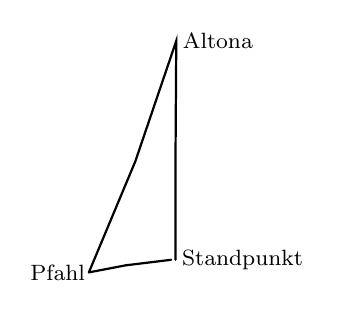
\begin{tikzpicture}[x=1mm,y=1mm,line width=.8pt,line cap=round]
  \coordinate (Pfahl) at (0,0);
  \coordinate (Altona) at (11.1,29.4);
  \coordinate (Standpunkt) at (11.0,1.6);
  \draw (Pfahl) -- (5.9,14.1) -- (Altona) -- (11.0,14.0) -- (Standpunkt);
  \draw (Pfahl) -- (4.7,.9) -- (10.45,1.6);
  \node[font=\footnotesize,anchor=east,inner sep=1pt] at (Pfahl) {Pfahl};
  \node[font=\footnotesize,anchor=west,inner sep=2pt] at (Altona) {Altona};
  \node[font=\footnotesize,anchor=west,inner sep=2pt] at (Standpunkt) {Standpunkt};
 \end{tikzpicture}
\end{minipage}\hfill
\begin{minipage}[t]{.71\linewidth}
 \vspace{0pt}
 \setlength{\parindent}{1.5em}
 \indent I,\quad Der Winkel in Altona zwischen den Richtungen nach dem Pfahl und Standpunkt;

 II.\quad eine kleine Correction wegen der Krümmung der Erde, welche bewirkt, dass der Unterschied der Richtung Altona-Standpunkt und Standpunkt-Altona nicht genau \(180^\circ\) ist. Beide Berichtigungen können
\end{minipage}\par
\noindent aber erst berechnet werden, wenn die Lage des Standpunkts schon näherungsweise wenigstens bekannt ist. Man mag diese also erst suchen, indem man jene beiden einstweilig ignorirt. Dazu bedarf es nun keiner Anleitung; Sie mögen nach Gefallen das \(\Delta\) Altona, Standpunkt, Hamburg oder Altona, Standpunkt, Rönneberg, etc. dazu anwenden. Ich bemerke nur, dass um I. zu berechnen, bloss die Entfernung Altona-Standpunkt nöthig ist; in obigem Dreieck sind dann 2 Seiten und ein Winkel bekannt. Ich finde nun
\[
\raisebox{\baselineskip}{\(\displaystyle
\left.
\begin{array}{@{}l@{\;=\;}l@{}}
 \log(\text{Altona-Standpunkt})&4{,}09915\\
 \log(\text{Standpunkt-Pfahl})&0{,}16643\\
 \text{Winkel [im] Standpunkt}&129^\circ36'58''
\end{array}\right\}
\)}
\begin{array}{@{}l@{\;}c@{\;}r@{}}
 \text{Der Winkel in Altona}&=&18''{,}551\\
 \text{und also, da in Altona}&&\\
 \text{Azimuth des Pfahls}&=&13^\circ\,34'\,20''{,}225,\\
 \cline{2-3}
 \text{ebendaselbst}&&\\
 \text{Azimuth des Standpunkts}&=&13^\circ\,34'\,1''{,}674.
\end{array}
\]

Ad II. bemerke ich, dass zu dieser Correction die genäherten Coordinaten vom Standpunkt erforderlich sind.

Sind die von Altona \(a,b\),\par
vom Standpunkt \(x,y\),\par
so ist die Correction \(=-A(x-a)(y+b)\),\par
\noindent wo \(A\) eine Grösse ist, die eigentlich Function von \(x\) ist, genauer von \(\frac12(x+a)\), aber sich sehr langsam ändert[*)].
\[
\begin{array}{@{}c@{\quad}l@{\quad}c@{\enspace}c@{\;=\;}l@{}}
 \text{Für}&\text{Altona}&\text{ist}&\log A&1{,}40336-10\\
 \text{»}&\text{Lysabbel}&\text{»}&\text{»}&1{,}40323-10.
\end{array}
\]
\indent Die Rechnung steht also so:
\[
\begin{array}{@{}r@{\;=\;}r@{\qquad}r@{\;=\;}r@{\enspace}l@{}}
 a&-224495{,}3&b&+16{,}4&\\
 x&-212281{,}4&y&+2963{,}7&\text{(sind übrigens schon gute Coordinaten)}
\end{array}
\]

\par\smallskip\noindent\rule{4cm}{.4pt}\par
{\footnotesize\noindent\hspace*{\parindent}[*) Vergl. S.~216/217, wo \(q\) für \(A\) geschrieben ist. Die Correction ist, wenn \(A\) für beide Punkte gleich angenommen wird: \(-A(x-a)\dfrac{2b+y}{3}+A(a-x)\dfrac{2y+b}{3}\).]\par}

% Printed 287; principal PDF 294; Google PDF 298.
\par\clearpage
\noindent\null\hfill{\small\textbf{STATIONSAUSGLEICHUNGEN.}}\hfill\makebox[0pt][r]{\fontsize{13}{16}\selectfont 287}\par\medskip

\[
\begin{array}{@{}r@{\;=\;}r@{\qquad}l@{\enspace}l@{}}
 x-a&+12213{,}9&\log.\,.\,.\,.\,.\,.&4{,}08686\\
 y+b&+2980{,}1&\log.\,.\,.\,.\,.\,.&3{,}47423\\
 \multicolumn{2}{c}{}&\log(-A).\, .&1{,}40336_n-10\\
 \cline{3-4}
 \multicolumn{2}{c}{}&&8{,}96445_n-10.
\end{array}
\]
\[
\begin{array}{@{}r@{\quad}c@{\;}l@{}}
 \text{Zahl}&=&\qquad-0''{,}092.\\[3pt]
 \text{Azimuth \textls[120]{in} Altona}&=&13^\circ\,34'\,1''{,}674\\
 &&180\\
 \cline{3-3}
 \text{Azimuth \textls[120]{von} Altona}&=&193^\circ\,34'\,1''{,}582.
\end{array}
\]
\indent Obiges Tableau bedarf also, um orientirt zu sein, einer Correction von \(-28''{,}394\) und steht also so:
\[
\begin{array}{@{}l@{\enspace}r@{\;}r@{\;}l@{}}
 \text{\hbox to 8.7em{Pfahl\hfil.\hfil.\hfil.\hfil.\hfil.\hfil.\hfil.\hfil.\hfil.}}&63^\circ&57'&4''\\
 \text{\hbox to 8.7em{Neuenfelde\hfil.\hfil.\hfil.\hfil.}}&148&22&31{,}267\\
 \text{\hbox to 8.7em{Altenwerder\hfil.\hfil.\hfil.}}&189&27&10{,}451\\
 \multicolumn{4}{c}{\text{etc.}}
\end{array}
\]

\begin{center}\rule{3cm}{.4pt}\end{center}
\vspace{.8cm}
\begingroup\small
\begin{center}
 BEMERKUNGEN.
\end{center}

Eine Zusammenstellung der endgültigen Ausgleichungen von Stationsbeobachtungen, deren Ergebnisse in die Netzausgleichung eingeführt sind, ist nicht vorhanden. Die Resultate der Stationsausgleichungen selbst sind mitgetheilt, Band IV, S.~449 u.~f., in den »Abrissen der auf den verschiedenen Stationen der Gradmessung, 1821, 1822, 1823, und deren Fortsetzung bis Jever, 1824, 1825, festgelegten Richtungen.« Doch zeigen die Richtungswerthe, welche \textsc{Gauss} für die Netzausgleichung benutzt hat (wie aus der Dreieckszusammenstellung der beobachteten Winkel im folgenden Abschnitt hervorgeht) noch kleine Abweichungen von jenen, die von den Reductionen wegen der Höhe des anvisirten Objects und wegen der Abweichung der geodätischen Linie vom Verticalschnitt herrühren (vergl. dazu den später folgenden Brief an \textsc{Olbers} vom 14. Mai 1826), bei manchen Richtungen aber auch noch in Centrirungsbeträgen ihren Grund haben müssen.

Die mitgetheilten Stationsausgleichungen für Zeven und Brillit, [1] und [2], die nicht die endgültigen sind, wurden einem Handbuche entnommen, in welches \textsc{Gauss} im Ganzen 8 Ausgleichungen von Stationsbeobachtungen eingetragen hatte. An Stelle der angegebenen Constanten in der dritten und vierten Normalgleichung für Zeven hatte \textsc{Gauss} irrthümlich \(+0{,}346\) und \(-1{,}189\); infolge dessen weicht sein Auflösungstableau von dem vorstehend gegebenen ab. Je nach dem Stande der Beobachtungen sind die Ausgleichungen von \textsc{Gauss} mehrmals wiederholt (vergl. S.~280, unten); so ist die hier mitgetheilte Ausgleichung für die Station Wilsede, Notiz [3], die vierte, die sich in einem Beobachtungs- und Rechnungshefte für die hannoversche Gradmessung befand. Ihr Ergebniss stimmt mit der Angabe unter den »Abrissen

% Printed 288; principal PDF 295; Google PDF 299.
\par\clearpage
\noindent\makebox[0pt][l]{\fontsize{13}{16}\selectfont 288}\hfill{\small\textbf{BEMERKUNGEN.}}\hfill\null\par\medskip

\noindent etc.«, Band IV, S.~454, überein, wenn man hier die Orientirung um \(-0''{,}665\) verändert. Berechnet man nach Art.~13, S.~95, für Wilsede die Correctionen der beobachteten Richtungen wegen der Meereshöhe des eingestellten Objects und wegen der Abweichung der geodätischen Linie vom Verticalschnitt, so erhält man für die Richtung nach Falkenberg (150,8 m): \(+0''{,}001\), nach Elmhorst (90,0 m): \(+0''{,}003\), für die Richtungen nach Steinberg (72,3 m), Bottel (52,4 m), Bullerberg (53,3 m), Brüttendorf (49,6 m) und Zeven (44,8 m) je \(0''{,}000\), für die Richtung nach Litberg (65,5 m): \(-0''{,}001\), nach Hamburg (144,9 m): \(0''{,}000\), nach Lüneburg (99,1 m): \(+0''{,}002\), nach Nindorf (116,7 m): \(-0''{,}001\), nach Timpenberg (117,1 m): \(-0''{,}002\), nach Wulfsode (104,5 m): \(-0''{,}003\), nach Breithorn (120,5 m): \(-0''{,}002\) und nach Hauselberg (120,4 m): \(-0''{,}002\). Die eingeklammerten Werthe der Meereshöhen sind einem \textsc{Gauss}schen Handbuche entnommen. Werden diese Correctionen an die Ausgleichungsergebnisse angebracht, so folgen die für Wilsede in die Netzausgleichung eingeführten Werthe.

Sämmtliche noch vorhandenen Stationsausgleichungen finden sich theils in kleinen Beobachtungs- und Rechnungsheften zur Gradmessung, theils auf losen Blättern zerstreut. Die Form der Ausgleichung ist bei allen Hauptdreieckspunkten so, wie bei Zeven oder Wilsede, in wenigen Fällen wie bei Brillit (vergl. die Briefe an \textsc{Olbers} vom Juli 1825, an \textsc{Schumacher} vom 14. August 1825 und an \textsc{Bessel} vom 29. October 1843).

Eine symmetrische Anordnung der Messungen hat auf keinem Hauptdreieckspunkte stattgefunden. Nur auf einigen Nebenpunkten scheinen alle Winkel-Combinationen beobachtet zu sein. Die Beobachtungen auf dem Windberge, Notiz [4], von dem Artillerie-Lieutenant F.~\textsc{Hartmann}, einem der Gehülfen \textsc{Gauss}' bei der Triangulation, geben ein Beispiel dafür. (Auf dem Original, einem einzelnen Blatte, ist von \textsc{Hartmann} noch hinzugefügt: »Wegen Abgang der Post nicht vollständig. Den Winkel \(7.3\) will ich noch einmal messen, vielleicht hat diese Wiederholung auch auf den Winkel \(3.5\) einen günstigen Einfluss«. Sie ist aber nach dem Beobachtungsbuche nicht erfolgt.) Die Messungen auf dem Windberge haben im Juni 1830 stattgefunden.

In welcher Weise \textsc{Gauss} beobachtet hat, zeigt der Auszug aus einem Beobachtungshefte für den Gradmessungspunkt Breithorn, Notiz [5].

Über das bei der hannoverschen Triangulation angewandte Verfahren gibt auch der nachfolgende Auszug aus dem bereits erwähnten Heftchen mit dem Titel: »Geodätischer Calcül nach \textsc{Gauss}« von Prof. \textsc{Goldschmidt} Auskunft. \textsc{Goldschmidt} hat \textsc{Gauss} wahrscheinlich, wie schon früher mitgetheilt ist, in den letzten Jahren der Landesvermessung bei den Rechnungen unterstützt; 1834 hat er bei dem Lieutenant \textsc{Gauss} an den Messungen für die Detailaufnahme Theil genommen.

»Bei der Triangulirung selbst wird zuerst eine mässige Anzahl von Punkten, die den aufzunehmenden Raum so bedecken, dass sie eine weite Aussicht haben, ausgewählt. Von diesen \textls[120]{Hauptpunkten} nimmt man nur so viele, als gerade nöthig sind, um die sogenannten Punkte zweiter Ordnung, von denen wir sogleich reden werden, zu bestimmen; ihre Entfernung wird übrigens so gross genommen, als das Terrain und die Stärke der anzuwendenden Fernrohre es nur irgend gestatten. Auf \textls[120]{jedem} der ausgewählten Hauptdreieckspunkte schneidet man nun alle überhaupt sichtbaren Objecte, deren Bestimmung mit im Plane liegt, ein, misst aber hauptsächlich die Winkel unter den übrigen hier sichtbaren Hauptpunkten mit vielfacher Repetition, ebenso misst man die Winkel zwischen den ausgewählten Nebenpunkten und den Hauptpunkten.

Die Hauptdreieckspunkte dienen dazu, dem ganzen Systeme eine feste Haltung zu geben, und deshalb wählt man nur wenige derselben, und nimmt lieber ihre Entfernung so gross als möglich, um weniger Zwischenstationen zu haben, bei denen sich die begangenen Fehler immer mehr und mehr anhäufen könnten.

Die geringe Menge der ausgewählten Hauptdreieckspunkte würde es uns aber unmöglich machen, alle von ihnen umschlossenen Punkte mit Genauigkeit zu bestimmen, selbst wenn das Terrain es verstattete,

% Printed 289; principal PDF 296; Google PDF 300.
\par\clearpage
\noindent\null\hfill{\small\textbf{STATIONSAUSGLEICHUNGEN.}}\hfill\makebox[0pt][r]{\fontsize{13}{16}\selectfont 289}\par\medskip

\noindent nach allen festzusetzenden Punkten zu visiren, denn es würde hiebei nicht zu vermeiden sein, dass viele Punkte durch sehr spitze Dreiecke bestimmt werden müssten, in denen bekanntlich ein sehr kleiner beim Messen der Winkel begangener Fehler die Lage des Punktes ungemein abändern würde. Dies ist der Grund, warum man noch eine grössere Anzahl von \textls[120]{Nebenpunkten} auswählt.

Diese wählt man so, dass sie 1) zur Bestimmung \textls[120]{aller} überhaupt festzusetzenden Punkte genügen, 2) dass sie \textls[120]{wo möglich} aus den Hauptdreieckspunkten sich mit \textls[120]{Schärfe} bestimmen lassen, wobei man indessen nicht zu ängstlich zu sein braucht, denn wenn ein solcher Punkt sich nicht aus Hauptdreieckspunkten bestimmen lässt, so kann man ihn durch Nebenpunkte bestimmen; doch ist es, der Orientirung halber, immer gut, wenigstens einen Hauptdreieckspunkt einzuschneiden. Übrigens schneidet man auch von den Nebenpunkten \textls[120]{alle überhaupt sichtbaren} Objecte, die mit bestimmt werden sollen, ein, die Haupt- und Nebenpunkte mit mehrfacher Repetition und Ablesung, die übrigen Punkte, welche keine Standpunkte sind, allenfalls nur einmal.

Dies ist die allgemeine Übersicht der Triangulation; jetzt einige ins Einzelne gehende Bemerkungen.\par
\noindent Durch Drehung des Alhidadenkreises wird immer eine, wenn auch geringe Drehung des eingetheilten Kreises herbeigeführt, und hiedurch können constante Fehler entstehen, dergestalt, dass man, beim Messen von der Linken zur Rechten, den Alhidadenkreis immer auf dem kürzesten Wege nach dem Object hin bewegend, die Winkel immer zu klein finden würde. (Bei der Discutirung der Messungen, die Lieutenant \textsc{Gauss} 1833 in Westphalen vorgenommen, habe ich den mittlern hieraus sich ergebenden Fehler etwa \(1''{,}5\), bei den Messungen vom Hauptmann \textsc{Müller} \(3''\) gefunden.) Um dies zu compensiren, führt \textsc{Gauss} den Alhidadenkreis ebenso oft auf dem kürzesten als auf dem längsten Wege in die Richtung des zweiten Objects.

\begin{center}
 \textls[120]{Messungen der Winkel von einem Standpunkte aus.}
\end{center}

Wir wählen zuerst einige Punkte aus, die eine für ein scharfes Pointiren geeignete Gestalt haben. Die Anzahl derselben darf, wenn man scharfe Resultate haben will, wohl nicht unter 4 und, wenn unnöthige Weitläufigkeit vermieden werden soll, nicht über 6 sein. Am gerathensten ist es, wenn dieselben Hauptpunkte des Systems sind und zu gleicher Zeit den Horizont in gleiche Theile theilen. Doch braucht man nicht zu ängstlich rücksichtlich dieser Bedingungen zu sein. Man misst nun die Winkel zwischen je zweien dieser Objecte, indem man alle möglichen Combinationen macht. Nachher gleicht man die gefundenen Werthe nach der Methode der kleinsten Quadrate aus. Jeden andern festzusetzenden Punkt vergleichen wir nun mit einer der so bestimmten Richtungen; wenn er schärfer bestimmt werden soll, durch mehrmalige Repetition, vielleicht auch vergleichen wir ihn mit zweien; geben diese nicht dasselbe Resultat, so wendet man auch hier die Methode der kleinsten Quadrate an. Wie dies geschieht, wollen wir sogleich angeben.

Die Anwendung der Methode der kleinsten Quadrate wollen wir an einem Beispiele zeigen. Vom Standpunkt \textls[120]{Hoheegge} wurden \textls[120]{Enegerloh} (1), \textls[120]{Dörenberg} (2), \textls[120]{Nonnenstein} (3), \textls[120]{Hünenburg} (4) als Vergleichungspunkte ausgewählt und folgende Winkel, jeder mit 20-maliger Repetition, gemessen:
\[
\begin{array}{@{}r@{\;=\;}r@{\;}r@{\;}l@{}}
 1.2&77^\circ&42'&38''{,}313\\
 1.3&162&40&2{,}500\\
 2.3&84&57&24{,}750\\
 3.4&107&59&41{,}375\\
 4.1&89&20&16{,}438\\
 4.2&167&2&53{,}025.
\end{array}
\]

Man nehme jetzt die Azimuthe der 4 Punkte 1, 2, 3, 4, d.~h. man beziehe alle auf eine und dieselbe Fundamentalrichtung; ob diese wirklich der Meridian ist, ist hiebei ganz gleichgültig, doch thut man wohl,
\par\smallskip\noindent\makebox[0pt][l]{\small IX.}\makebox[.86\linewidth][r]{37}\par

% Printed 290; principal PDF 297; Google PDF 301.
\par\clearpage
\noindent\makebox[0pt][l]{\fontsize{13}{16}\selectfont 290}\hfill{\small\textbf{BEMERKUNGEN.}}\hfill\null\par\medskip

\noindent diese Richtung nicht allzuweit vom Meridian zu entfernen, um nachher keine zu grosse Correction wegen der Orientirung anbringen zu müssen. Näherungsweise kann man sich ja immer die Richtung des Meridians allenfalls mit der Boussole verschaffen (wie \textsc{Hartmann} dieses auf dem Harze da that, wo er kein Azimuth kannte). Ein genäherter Werth des Azimuths von 1 ist \(41^\circ25'0''{,}0\); wären alle Winkel, von denen 1 ein Schenkel ist, richtig gemessen, so wären die Azimuthe von
\[
\begin{array}{@{}r@{\;=\;}r@{\;}r@{\;}l@{}}
 2&119^\circ&7'&38''{,}313\\
 3&204&5&2{,}500\\
 4&312&4&43{,}562.
\end{array}
\]

Berechnet man z.~B. 3 nicht aus 1 und \(1.3\), sondern aus 2 und \(2.3\), so findet man \(3=2+2.3=204^\circ5'3''{,}063\), also von dem oben angegebenen Werthe verschieden; wir müssen also bei 2, 3, 4 noch Correctionen anbringen. 2, 3, 4 sind nur genähert, und wir lassen der leichtern Rechnung halber die Decimaltheile der Secunde weg, indem wir diese mit in der Correction enthalten sein lassen; dann ist
\[
\begin{array}{@{}r@{\;=\;}r@{\;}r@{\;}r@{\;}l@{}}
 1&41^\circ&25'&0''{,}0&\\
 2&119&7&38{,}0&+x\\
 3&204&5&2{,}0&+y\\
 4&312&4&43{,}0&+z.
\end{array}
\]

Berechnet man hieraus die Winkel, so ist:
\[
\begin{array}{@{}r@{\;=\;}r@{\;}r@{\;}r@{\;}l|r|r@{\;}l@{\;=\;}l@{}}
 \multicolumn{5}{c}{\text{Calc.}}&
 \multicolumn{1}{c}{\text{Obs.}}&
 \multicolumn{3}{c}{\text{Obs.-Calc.}}\\
 1.2&77^\circ&42'&38''{,}0&+x&38''{,}313&-0''{,}313&+x&\varepsilon'\\
 1.3&162&40&2{,}0&+y&2{,}500&-0{,}500&+y&\varepsilon''\\
 2.3&84&57&24{,}0&-x+y&24{,}750&-0{,}750&-x+y&\varepsilon'''\\
 3.4&107&59&41{,}0&-y+z&41{,}375&-0{,}375&-y+z&\varepsilon^{\mathrm{IV}}\\
 4.1&89&20&17{,}0&-z&16{,}438&+0{,}562&-z&\varepsilon^{\mathrm{V}}\\
 4.2&167&2&55{,}0&+x-z&53{,}025&+1{,}975&+x-z&\varepsilon^{\mathrm{VI}}
\end{array}
\raisebox{-.5\baselineskip}{%
 \(\left.\vphantom{\begin{array}{c}0\\0\\0\\0\\0\\0\end{array}}\right\}\)%
 \enspace\rotatebox[origin=c]{-90}{Fehlergleichungen.}%
}
\]

Bildet man hieraus nach der Methode der kleinsten Quadrate die Fundamentalgleichungen, so ist
\[
\begin{array}{@{}r@{\;}r@{\;}r@{\;}r@{\;=\;}l@{}}
 +2{,}412&+3x&-y&-z&0\\
 -0{,}875&-x&+3y&-z&0\\
 -2{,}912&-x&-y&+3z&0.
\end{array}
\]

Gleichungen dieser Form lassen sich am besten auf folgende Art lösen; addirt man sie, so ist
\[
 -1{,}375+x+y+z=0,
\]
und addirt man diese zu jeder einzelnen Fundamentalgleichung, so kommt:
\[
\begin{array}{@{}r@{\;}l@{\;=\;}r@{\qquad}c@{\;=\;}l@{}}
 +1{,}037&+4x&0&x&-0{,}259\\
 -2{,}250&+4y&0&y&+0{,}563\\
 -4{,}287&+4z&0&z&+1{,}072.
\end{array}
\]

Diese leichte Eliminationsmethode lässt sich bei den symmetrischen Fundamentalgleichungen, auf welche diese Aufgabe jedesmal führt, wenn alle Combinationen unter den Richtungen und zwar alle mit gleicher Repetition gemessen sind, jedesmal anwenden. Wir finden also die verbesserten Azimuthe:

% Printed 291; principal PDF 298; Google PDF 302.
\par\clearpage
\noindent\null\hfill{\small\textbf{STATIONSAUSGLEICHUNGEN.}}\hfill\makebox[0pt][r]{\fontsize{13}{16}\selectfont 291}\par\medskip

\[
\begin{array}{@{}l@{\quad}r@{\;}r@{\;}r@{\quad}l@{\quad}r@{\quad}r@{\;}r@{\;}r|l@{}}
 \multicolumn{6}{c}{}&\multicolumn{3}{c}{\text{Calc.}}&\multicolumn{1}{c}{\text{Calc.-Obs.}}\\
 1.&41^\circ&25'&0''{,}000&&1.2&77^\circ&42'&37''{,}741&-0''{,}572\\
 2.&119&7&37{,}741&&1.3&162&40&2{,}563&+0{,}063\\
 3.&204&5&2{,}563&&2.3&84&57&24{,}822&+0{,}072\\
 4.&312&4&44{,}072&\text{und hieraus}&3.4&107&59&41{,}509&+0{,}134\\
 &&&&&4.1&89&20&15{,}928&-0{,}510\\
 &&&&&4.2&167&2&53{,}669&+0{,}644.
\end{array}
\]

Sind die Winkel nicht alle mit einer gleichen Anzahl Repetitionen gemessen, so dass sie also verschiedene Gewichte haben, so muss man jeden Beitrag der Fehlergleichungen für \(\varepsilon',\varepsilon'',\varepsilon''',\ldots\) zu den Fundamentalgleichungen mit dem Gewicht, d.~h. mit der Zahl, welche der Anzahl der Repetitionen proportional ist, multipliciren. Um auch hierüber ein Beispiel anzuführen, nehmen wir die von [Lieutenant] \textsc{Gauss} in \textls[120]{Neuenkirchen} gemessenen Winkel.

\begin{center}
 1. Dörenberg\qquad 2. Quekenberg\qquad 3. Quackenbrück\qquad 4. Mordkuhlenberg.
\end{center}

Er fand
\[
\begin{array}{@{}r@{\quad}r@{\;}r@{\;}r@{\quad}c@{\qquad}l@{\quad}r@{\;}r@{\;}r@{\;}l@{}}
 \multicolumn{4}{c}{}&\text{Pond.}&
 \multicolumn{5}{c}{\text{Azimuthe}}\\
 1.2&93^\circ&9'&2''{,}875&5&1.&6^\circ&25'&58''{,}000&\quad\text{[*)]}\\
 1.3&147&10&10{,}938&1&2.&99&35&0{,}875&+b\\
 2.3&54&1&4{,}125&5&3.&153&36&5{,}656&+c\\
 3.4&86&21&14{,}875&5&4.&239&57&22{,}453&+d\\
 4.1&126&28&33{,}625&5&&&&&\\[3pt]
 &\multicolumn{3}{c}{\text{Calc.-Obs.}}&\text{Pond.}&&&&&\\
 1.2&&&0''{,}000+b&5&&&&&\\
 1.3&&&-3{,}282+c&1&&&&&\\
 2.3&&&+0{,}656-b+c&5&&&&&\\
 3.4&&&+1{,}922-c+d&5&&&&&\\
 4.1&&&+1{,}922-d&5.&&&&&
\end{array}
\]

Bildet man die Fundamentalgleichungen, indem man die Beiträge der obigen Fehlergleichungen mit ihren resp. Gewichten multiplicirt, so findet man
\[
\begin{array}{@{}r@{\;}c@{\;}r@{\;}c@{\;=\;}l@{}}
 -3{,}280&+10b&-5c&*&0\\
 -9{,}612&-5b&+11c&-5d&0\\
 \multicolumn{1}{c@{\;}}{0}&*&-5c&+10d&0,
\end{array}
\]
und jetzt werden nach bekannten Regeln \(b,c,d\) gefunden, und damit die obigen Werthe der Azimuthe verbessert.

Hat man auf diese Art die zwischen den Hauptrichtungen gemessenen Winkel ausgeglichen, so bestimmt man mit ihnen die übrigen, die, wie schon gesagt, beim Einschneiden mit einer der angenommenen Hauptrichtungen verbunden werden. Ist z.~B. ein Punkt \(A\) mit der Hauptrichtung 1, deren Azimuth wir 1 nennen, verbunden, indem der Winkel \(1.A\) gemessen ist, so haben wir das Azimuth von \(A=1+1.A\);

\par\smallskip\noindent\rule{4cm}{.4pt}\par
{\footnotesize\noindent\hspace*{\parindent}[*) In einem Vorlesungsheft über höhere Geodäsie, das dieses Beispiel auch enthält, ist der Richtung nach 1 gleichfalls eine Verbesserung gegeben, so dass die Summe der Normalgleichungen gleich Null wird.]\par}
\par\smallskip\noindent\makebox[.86\linewidth][r]{37\textsuperscript{*}}\par
\endgroup
